\chapter{Opis implementacji}
\label{Chapter6}

\section{Wstęp}
\label{Chapter61}

Realizacja projektu iQuest rozciągała się na okres trwający 5 miesięcy. W tym czasie zrealizowano dwa kolejne wydania. \\

W pierwszym miesiącu -- w trakcie praktyk studenckich odbywanych przez 3 spośród 4 członków zespołu programistów -- utworzono pierwszą wtyczkę do platformy Moodle. Był to moduł logowania przez eKonto. Następne 3 miesiące trwało utworzenie pierwszego wydania, obejmującego podstawowe mechanizmy tworzenia badań i ankiet, oraz ich przeprowadzania. Ostatni miesiąc poświęcony został na dopracowanie wcześniej wspomnianych modułów o dodatkowe elementy, bezpośrednio związane z wymaganiami funkcjonalnymi i pozafunkcjonalnymi wyznaczonymi dla projektu. \\

W trakcie realizacji, zdarzały się dynamiczne zmiany podejścia do poszczególnych elementów systemu, co skutkowało zatwierdzaniem nowych decyzji projektowych i wymagało przebudowania gotowych już elementów. Dla zespołu programistów, było to bardzo trudne i wymagało poświęcenia znaczących nakładów czasowych. \\

W dalszej części niniejszego rozdziału znajduje się analiza systemu iQuest w kontekście implementacji. Rozpoczęty opisem napotkanych problemów i zastosowanych rozwiązań wywód, kontynuowany będzie opisem zastosowanych technologii. Wówczas nastąpi przejście do wyjaśnienia kwestii związanych z implementacją interfejsu i logiki, a także mechanizmów wiążących je ze sobą.

\section{Napotkane problemy i ich rozwiązania}
\label{Chapter62}

\subsection{Wstęp}
\label{Chapter621}
%KB

Problemy oraz ich rozwiązania zostały posortowane chronologicznie, zgodnie z kolejnością, w jakiej pojawiały się w czasie realizacji projektu. Celem ułatwienia ich analizy, wcześniej zamieszczono krótki wstęp teoretyczny opisujący budowę platformy \textit{Moodle}.

\subsection{Platforma Moodle}
\label{Chapter622}
%KU

Po zalogowaniu do systemu użytkownik musi wybrać \textit{kurs}. Jest on największą częścią platformy \textit{Moodle} i przeważnie kojarzony jest z ,,przedmiotem''. Na kurs składa się kilka lub kilkanaście \textit{sekcji}. Odpowiadają one najczęściej konkretnym zajęciom, wydarzeniom lub np.~tygodniom. Najmniejszą jednostką w Moodle jest \textit{aktywność}, będąca podstawowym typem modułów rozszerzających funkcjonalność platformy. Aktywnościami są np.~\textit{Fora}, \textit{Głosowania}, czy \textit{Czat}. \\

Istnieje również inny typ modułów: \textit{zasoby}. Są to m.in.~własne strony internetowe, pliki, adresy \definicja{URL}. Na potrzeby projektu została wyróżniona grupa \textit{materiały}. Zalicza się do niej wszystkie moduły inne niż \textit{iQuest}, czyli inne niż badania i związane z nimi ankiety. Moduły grupowane są w sekcje. Różnica pomiędzy tym, czy użytkownik znajduje się lub nie, w konkretnym elemencie platformy, jak moduł, czy kurs, nazywana jest \textit{kontekstem}. O ułożeniu i wyświetlaniu elementów na stronie decyduje \textit{formater}, definiując w ten sposób interfejs użytkownika.

\subsection{Inicjalizacja bazy danych}
\label{Chapter623}

Moduł \textit{iQuest} do prawidłowego działania wymaga rozszerzenia istniejącej bazy danych platformy \textit{Moodle} o dodatkowe tabele, przechowujące niezbędne do spełnienia założonej funkcjonalności dane. \\

Do zaimportowania bazy danych przygotowanej przez Architekta, wykorzystano narzędzie wbudowane w platformę Moodle: \textit{XMLDB}. Gwarantuje ono bezobsługową instalację modułu w przyszłości. W trakcie pracy z tym narzędziem, znaleziony został błąd, uniemożliwiający zaimportowanie kluczy obcych do bazy. W efekcie, programiści musieli ręcznie utworzyć wszystkie klucze obce, przewidziane przez Architekta, co wymagało znaczących nakładów czasowych.

\subsection{Instalacja modułu}
\label{Chapter624}
Postanowiono, że wraz z instalacją modułu \textit{iSurvey}, zawierającego logikę systemu \textit{iQuest}, powinien automatycznie tworzyć się powiązany z nim kurs. Rozwiązanie to zmniejsza nakład czasu wymagany do przygotowania platformy do użytku, oraz zapobiega pomyłkom związanym z ręcznym tworzeniem i konfiguracją systemu. \\

Konsekwencje takiego podejścia wyszły na jaw dopiero po jego zrealizowaniu. Okazało się, że podejście to uniemożliwia instalację modułu jednocześnie z całą platformą \textit{Moodle}, ponieważ w trakcie procesu instalacji platformy \textit{Moodle}, dodatkowe moduły instalowane są przed mechanizmami pozwalającymi na tworzenie \textit{kursu}. Z tego względu, moduł \textit{iSurvey} należy dodawać do wcześniej zainstalowanej platformy.
\subsection{Formularze}
\label{Chapter625}

Projektując graficzny interfejs użytkownika, prędzej czy później, pojawia się potrzeba wyboru narzędzia do projektowania formularzy. Rozważano kilka możliwości. Pierwszym, najbardziej naturalnym odruchem, była idea zastosowania czystego języka \textit{HTML}. Pod uwagę brane było także zastosowanie wbudowanych w \textit{Moodle} interfejsów programowania (ang. \definicja{Application Programming Interface, API}) -- \textit{Form API} oraz \textit{Output API} -- jak też użycie zewnętrznych \textit{API}, nie związanych bezpośrednio z platformą. \\

Zastosowanie \textit{HTML} oraz zewnętrznych \textit{API} zostało odrzucone. Decyzję tę podjęto ze względu na obawę, że pisanie interfejsu w całości od nowa okaże się zbyt pracochłonne. Z uwagi na dość mocno ograniczony czas, nie chciano wyważać otwartych już drzwi, tworząc coś, co już wcześniej zostało przez kogoś zrealizowane, nawet za cenę tego, że interfejs nie wyglądał dokładnie tak, jak go zaprojektowano -- na pierwszym miejscu stawiano jego kompletność. Zastosowanie zewnętrznych \textit{API} było natomiast niezgodne z założeniem, nakazującym stosowanie interfejsów \textit{Moodle} wszędzie tam, gdzie to możliwe. Użytkownik powinien mieć uczucie, że programowana wtyczka jest integralną częścią platformy. Co więcej, różnice w stosunku do oryginalnego wyglądu platformy mogłyby sprawić, że interfejs oceniony zostałby jako nieintuicyjny. To zaważyło na decyzji odnośnie zastosowania \textit{Output API} wbudowanego w \textit{Moodle}. \\

Wyżej wspomniane \textit{API} jest zestawem funkcji, wprowadzonych wraz wersją $2.0$ Moodle. Umożliwiają one wstawianie na stronę standardowych elementów formularza, takich jak: etykiety, przyciski, linki, tabele, itp. Niestety, z przyczyn nieznanych dla osób tworzących ten dokument, to doskonale wyposażone i w pełni udokumentowane \textit{API}, zostało usunięte z \textit{Moodle} wraz z aktualizacją do wersji $2.2$. Co jeszcze bardziej niezrozumiałe, część elementów można stosować w dalszym ciągu, lecz brak jest dokumentacji, określającej m.in.~których z nich to dotyczy. \\

Ostatecznie, realizacja interfejsu musiała odbyć się z użyciem \textit{Form API}. Ku rozczarowaniu zespołu programistów, ma on znacznie uboższą dokumentację. Zdarza się, że w funkcji są omówione np. tylko trzy pierwsze argumenty, podczas gdy reszta jest pominięta -- tak, jakby kompletnie nie istniała. \textit{Form API} różni się też od poprzednich \textit{API} tym, że jest oparte na modelu obiektowym. To sprawia, że zawiera szereg zalet, jak np.~fakt posiadania mechanizmu pozwalającego na weryfikację danych wprowadzanych przez użytkownika z użyciem \textit{JavaScript}. Mechanizm ten waliduje dane po stronie klienta, pozwalając na przesłanie do serwera jedynie poprawnych informacji. \\

Podsumowując, mimo niekompletnej dokumentacji, jako narzędzie implementacji formularzy wybrano \textit{Form API}. Choć zawiera ono sporo zalet, nie wszystkie potrzebne elementy udało się stworzyć korzystając jedynie z niego. Stosowano wówczas język \textit{HTML}. 

\subsection{Role}
\label{Chapter626}

Jedną z cech projektu, jest podział użytkowników na ankieterów i respondentów. W systemie \textit{Moodle} istnieje mechanizm do zarządzania rolami, który wydawał się adekwatny do użycia w tym przypadku. Rola jest to zbiór \textit{możliwości} (ang. \definicja{capability}), które można rozumieć, jako prawa do wykonania, fragmentu kodu określonego przez programistę. Zdecydowano więc o zastosowaniu tego gotowego rozwiązania.

\subsection{Formater kursu}
\label{Chapter627}

Jednym z problemów jakie napotkano, była konieczność wyświetlania respondentom i ankieterom tylko określonych modułów. Ankieterzy powinni zobaczyć tylko te badania, które utworzyli, lub które im udostępniono, wraz z innymi aktywnościami i zasobami. Respondenci powinni natomiast zobaczyć tylko te badania, w których mogą wziąć udział, a także materiały, do których pozyskali prawa do ich odczytu. \\

Do rozwiązania problemu zdecydowano się użyć formatera kursu. Narzędzie to, jako integralna część \textit{Moodle}, wydawało się najlepszym rozwiązaniem spośród dostępnych. W krótkim czasie okazało się jednak, że niekompletność dokumentacji, czy nawet merytorycznych dyskusji na ten temat w Internecie, znacząco utrudnia wykonanie zadania. Całą pracę wejścia, polegającą na poznaniu narzędzia, wykonano studiując kod źródłowy domyślnych formaterów dostępnych w \textit{Moodle}. \\

Pierwotnie zakładano wyświetlanie użytkownikowi dwóch sekcji. Jednej z odpowiednimi badaniami, drugiej z materiałami. Należało także ograniczyć ankieterowi możliwość dodawania w pierwszej sekcji modułów innych niż \textit{iQuest}, oraz dokładnie odwrotnego działania w drugiej z nich. Okazało się to nieosiągalne bez ingerowania w wewnętrzny kod platformy. \\

Przyczyną były uaktualnienia zastosowane w \textit{Moodle}. Kod \textit{PHP} wyświetlania typów modułów jest nadpisywany przez \textit{JavaScript}. W ten sposób, z poziomu funkcji \textit{PHP} odpowiedzialnych za wyświetlanie listy modułów w danej sekcji, nie da się kontrolować, które moduły zostaną wyświetlane, a które nie. Mówiąc prościej, programista może jedynie wybrać, jakie moduły będą wyświetlane we wszystkich sekcjach w danym kursie, nie mając wpływu na to, co można wykonywać w każdej sekcji z osobna. \\

Rozwiązaniem było umieszczenie listy badań oraz listy materiałów w jednej sekcji. Można w niej dodać jakikolwiek moduł. Dopiero przy wyświetlaniu moduły dzielone są na dwie listy: listę badań i listę materiałów. Dzięki temu cel został osiągnięty -- użytkownik zobaczy tylko te moduły, które ma prawo wyświetlać. Co więcej, będą one odpowiednio posegregowane, aby użytkownik szybko mógł znaleźć to, czego szuka.

\subsection{Tworzenie badania}
\label{Chapter628}

Kolejną trudnością w projekcie było połączenie utworzonej dla systemu \textit{iQuest} wtyczki z platformą \textit{Moodle}. Głównie sprowadzało się to do wykorzystania interfejsu graficznego \textit{Moodle} w sposób niwelujący uczucie zmiany systemu u użytkownika. Zarówno wygląd, jak i sposób wykorzystywania funkcjonalności, powinny być zgodne ze standardem \textit{Moodle}. Dzięki takiemu podejściu, osoba korzystająca wcześniej z platformy, a pragnąca używać wtyczki \textit{iQuest}, nie będzie musiała zmieniać swoich przyzwyczajeń. Co więcej, w projekcie duży nacisk postawiono na zachęcanie respondentów do wypełnienia ankiety, co było dodatkową motywacją do zaprojektowania przyjaznego użytkownikom interfejsu. \\

Wstępna wersja interfejsu, zaprojektowana przez Architekta, działała wedle następującego schematu: ankieter wyrażał chęć utworzenia nowego badania poprzez kliknięcie odpowiedniego przycisku. Wówczas mógł dodać do badania ankietę z katalogu, ewentualnie utworzyć nową. W kolejnych krokach, użytkownik definiował szczegóły badania, takie jak: nazwa, grupa docelowa, czas rozpoczęcia i zakończenia itp. Niestety, realizacja takiego rozwiązania okazała się niemożliwa. \\

Problem stwarzało dodawanie ankiety w trakcie procesu tworzenia badania, jeszcze przed jego zakończeniem. Zaczynając generowanie badania od zdefiniowania ankiety, nie można było jej od razu do niego dodać -- badanie to bowiem jeszcze nie istniało. W takim wypadku należałoby przechowywać informację, że po utworzeniu badania ma dodać się do niego ankieta\footnote{Przykładowo można w tym celu wykorzystać dodatkowy parametr w adresie \textit{URL}, choć stwarzałoby to potencjalny problem dotyczący kwestii liczby przekierowań, przez które musiałby on być przekazywany.}. Dodatkowo, w Moodle, przy kreowaniu nowego modułu, użytkownikowi wyświetlany jest domyślny formularz, w którym podaje się parametry potrzebne do zbudowania instancji tego modułu. Przyjmując, że badanie jest kojarzone z modułem, nie ma możliwości, aby przed zakończeniem tworzenia badania wstawić wewnątrz dodatkowy formularz. \\

Z tego względu, zamieniona została kolejność tworzenia badania i ankiety. Najpierw użytkownik tworzy badanie, czyli moduł realizujący ankietę. Dopiero wówczas ma możliwość załączenia do niego ankiety. Podejście to ma kilka zalet: jest to zgodne z procedurami charakterystycznymi dla \textit{Moodle}, a co za tym idzie, bardziej intuicyjne dla użytkownika obeznanego z platformą, a jednocześnie pozwala na łatwe dodanie ankiety do badania. Ponadto ankieter może zrezygnować z komponowania ankiety przy kreowaniu badania, odkładając to, znacznie bardziej czasochłonne, zadanie na później.

\subsection{Tworzenie ankiety}
\label{Chapter629}

Przy tworzeniu ankiety pojawił się dość specyficzny problem implementacyjny. Wynikał on z faktu, że ankietę definiować można zarówno z poziomu kursu, jak i z poziomu badania. Powstało pytanie: Jak przetwarzać dane pochodzące z różnych, niezależnych od siebie kontekstów? \\

Standardowo, we wtyczkach \textit{Moodle}, elementy odpowiedzialne za wyświetlanie informacji na ekranie znajdują się w pliku \textit{view.php}. Pojawił się pomysł, aby rozszerzyć strukturę o dwa dodatkowe pliki: \textit{mod.php} oraz \textit{course.php}. Do \textit{mod.php} trafiać miały dane z kontekstu modułu. Drugi plik zajmować miałby się przetwarzaniem danych z kontekstu kursu. Taki podział gwarantował większy porządek w kodzie źródłowym. Porządek był ważny, ponieważ \textit{Moodle} nie jest zgodny ze wzorcem Model-View-Controller. W związku z tym istotne jest aby efektywnie zarządzać kodem źródłowym, żeby mała jego zmiana nie wymagała zmiany wielu elementów. \\

Niestety wprowadzone zmiany okazały się niewystarczające. Występowało niepotrzebne powielanie kodu. Wydzielono jeszcze jeden plik, w którym przetwarzano dane otrzymane z formularzy i zapisywano je do bazy danych. Później zwracano sterowanie do wyżej wspomnianych plików, w zależności od kontekstu. \\

Dzięki utworzeniu trzech dodatkowych plików, kod źródłowy stał się bardziej przejrzysty. Wartość takiego rozwiązania można zauważyć dopiero, gdy zachodzi konieczność znalezienia błędu lub wprowadzenia modyfikacji do kodu. Przy dobrym zarządzaniu kodem mała zmiana wymaga nieznacznych tylko poprawek.

\subsection{Hierarchia CSS}
\label{Chapter62a}

Na wielu poziomach serwisu borykano się z problemem hierarchii plików \textit{CSS}. Twórcy platformy \textit{Moodle} po, jak zapewniają, gruntownym przemyśleniu sprawy i rozważeniu wszystkich możliwości, ustalili następującą hierarchię kaskadowych arkuszy stylów:

\begin{itemize}
\item Najważniejsze są pliki umieszczone w katalogu \textit{theme}, odnoszące się do całej platformy.
\item Następnie uwzględniane są reguły z pliku \textit{styles.css}, umieszczonego w katalogu konkretnej wtyczki.
\end{itemize}

Główną wadą tego podejścia jest fakt, że nie można we wtyczce nadpisać właściwości, która została zdefiniowana w katalogu \textit{theme}. Aby zmienić choćby jedną właściwość z tego katalogu należy utworzyć nowy \definicja{wygląd}, kopiując oryginalny i zmieniając tę jedną właściwość. Następnie administrator platformy musi ustawić ten wygląd w swoim systemie (co wiąże się z dodatkową operacją, jeśli poprzedni wygląd był wyglądem domyślnym). Ostatecznie jednak, problem ten udało się rozwiązać, stosując w tym celu atrybut \textit{!important}.

{\color{red}Fragment niezredagowany}

\subsection{Testy jednostkowe i akceptacyjne}
\label{Chapter 62b}

Realizacja wszystkich testów została pierwotnie powierzona jednemu z członków zespołu programistów. Zadanie to okazało się posiadać bardzo wysoki stopień złożoności, sprawiając, że napisanie pojedynczej linii kodu zajmowało średnio bardzo dużo czasu. \\

Przyczyną takiego stanu był stały rozwój systemu. Realizowany bez zastosowania metody rozwoju w oparciu o testowanie, iQuest z przerażającą szybkością ewoluował. Nowe parametry, nowe wartości wyjściowe oraz zmiana dostępności poszczególnych funkcji sprawiały, że utrzymywanie testów zajmowało nawet kilkudziesięciokrotnie więcej czasu, niż ich utworzenie od nowa. \\

Problem ten występował jednak jedynie w trakcie pierwszego wydania projektu. Przy drugim wydaniu, działalność związaną z testami jednostkowymi w sporej mierze przejął programista logiki aplikacji, co znacząco zmniejszyło czasochłonność ich realizacji. \\

Większy problem tyczył się testów akceptacyjnych. Już na początku realizacji projektu, wyszło na jaw, że eksport z Selenium IDE (standard HTML) do Eclipse IDE (standard Java) nie jest zadaniem prostym. Dla przykładu, część metod odwołania do poszczególnych obszarów na stronie nie może być przenoszony do Javy, ze względu na znane problemy. \\

Na podstawie powyższej analizy stwierdzono, że testy akceptacyjne mogą być wykonywane za pomocą rozszerzenia Selenium IDE for Firefox, szczególnie, że narzędzia w nim dostępne umożliwiają spory stopień automatyzacji.

\subsection{Mapowanie obiektowo-relacyjne}
\label{Chapter62c}
%LW

Mapowanie obiektowo-relacyjne pozwala uprościć operacje na danych przechowywanych w bazie danych poprzez udostępnienie ich programiście w postaci obiektowej. \\

System \emph{iQuest} operuje na klasach takich jak: ankieta, badanie, grupa docelowa, członek grupy docelowej, uprawnienie dostępu, pytanie (i potomne), odpowiedź, zadanie, praca w tle, etc. Początkowo architekt stworzył diagram klas na którym każda klasa miała wyróżnione publiczne metody \emph{insert, update, delete}. Niestety takie rozwiązanie spowodowało powielenie dużej ilości kodu związanego z interakcją z bazą danych. W ramach refaktoryzacji podjąłem się zadania stworzenia klas, które wzorem nowoczesnych systemów \emph{ORM} uproszczą projektowanie nowych klas reprezentujących dane. Ze względu na silną integrację z mechanizmami \emph{Moodle} w grę nie wchodziły gotowe rozwiązania. Autorskie rozwiązanie korzysta z mechanizmów \emph{Moodle Data manipulation API} oraz mechanizmu refleksji języka PHP, by pozwolić programiście korzystającego z tego rozwiązania na proste pobieranie i manipulację obiektami przechowywanymi w bazie danych. Diagram UML przedstawia się następująco:

\begin{figure}[H]
\begin{center}
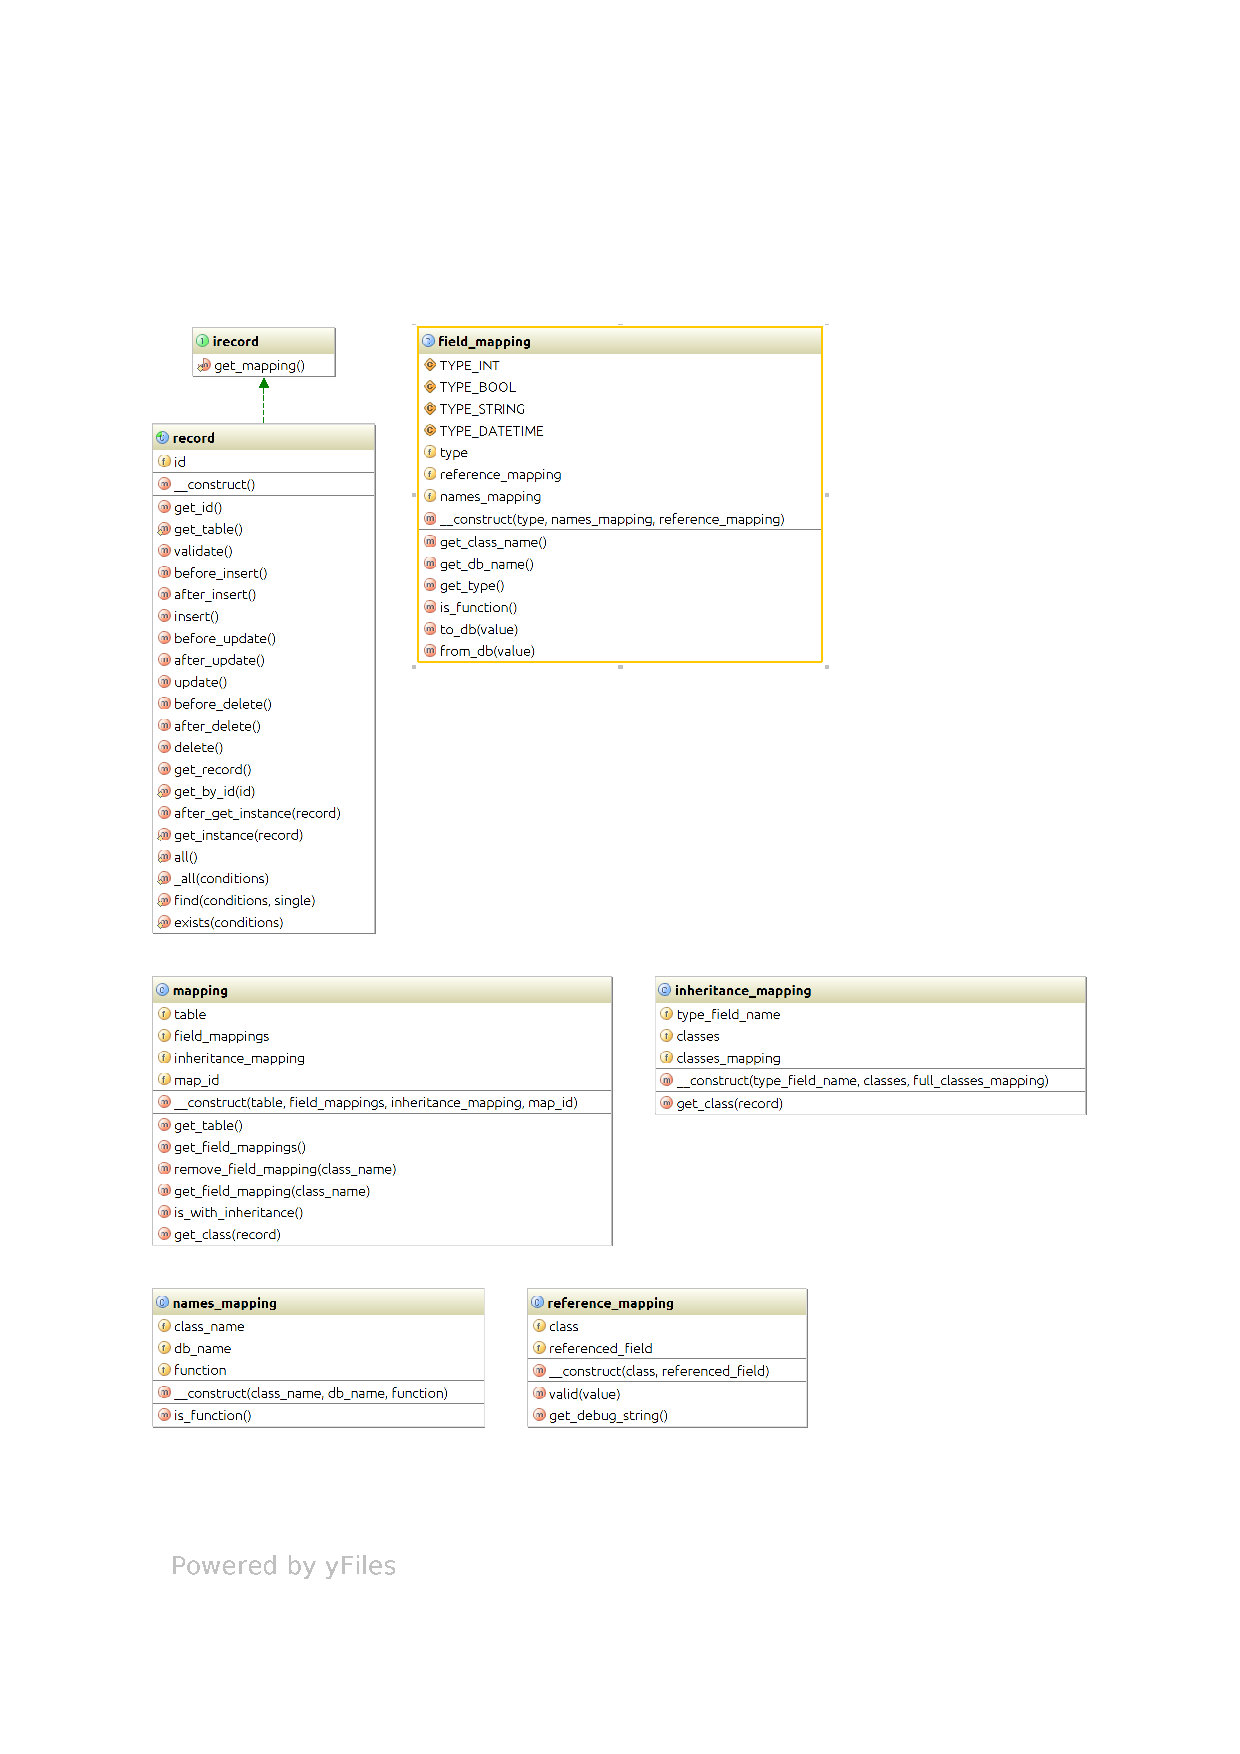
\includegraphics[width=0.9\textwidth]{figures/lw/orm.pdf} 
\end{center}
\caption{iQuest ORM}\label{fig:iquest-orm}
\end{figure}

Klasa danych dziedziczy po klasie \emph{record} oraz implementuje metodę \emph{get\_mapping} interfejsu \emph{irecord}, by uzyskać dostęp do metod komunikacji z bazą danych. Metoda \emph{get\_mapping} pozwala zdefiniować mapowanie danej klasy na odpowiednią relację w bazie danych. Należy przy tym podać mapowania dla atrybutów, tj. nazwy w klasie i bazie danych oraz typ, który zadecyduje o metodzie pobrania/zapisania danej (typem może być także klasa potomna klasy \emph{record}). W przypadku, gdy mamy do czynienia z dziedziczeniem wystarczy zdefiniować przy mapowaniu sposób obsługi dziedziczenia (m.in. jakie pole określa typ klasy). Najważniejszy kod znajduje się w metodzie \emph{get\_instance}, która pobiera konstruktor danej klasy, poprzez refleksję tworzy obiekt z wyłuskanymi z bazy danych parametrami wymaganymi przy jego tworzeniu oraz ustawia resztę pól pobranych z bazy danych. Metody \emph{insert, update, delete} pobierają reprezentację obiektu oczekiwanego przez metody \emph{Data manipulation API} oraz wykonują żądane operacje.\\
Zastosowane rozwiązanie znacząco poprawiło czytelność kodu poprzez zastosowanie zasady DRY (\emph{Don't repeat yourself}). Projektowałem je, mając na uwadze rozwiązanie, z którym miałem wcześniej styczność, tj. implementację \emph{ActiveRecord} z \emph{Ruby on Rails}. W trakcie pracy nad projektem doceniłem stosowanie konwencji nazewniczych, których obecność znacząco upraszcza projektowanie klas mapujących dane.

\subsection{Inwencja programistów}
\label{Chapter62d}

W trakcie rozwoju oprogramowania pojawiło się kilka małych niejasności, które należało rozwiązać. Kilka razy wykazano również inicjatywę i zaproponowano rozwiązania, które stały się ostatecznie częścią projektu.

Pierwszą ideą było zagospodarowanie przestrzeni w widoku badania. Po utworzeniu badania i dodania do niego ankiety, ankieterowi ukazuje się widok badania. Architekt nie zaproponował jak ma on wyglądać. Dał tylko pewne wskazówki. Zaznaczył, że z tego widoku, ankieter ma mieć możliwość usunięcia ankiety z badania oraz edytowania jej. I tu pojawił się problem. Żeby spełnić wymagania, na stronie wystarczyło pokazać odnośniki: ,,edytuj'' i ,,usuń z badania''. Praktycznie cała strona pozostawała pusta. Sytuacja taka jest niedopuszczalna, bo na pewno istniały jakieś przydatne informacje, które można było w tym miejscu wyświetlić. Wykoncypowano, że najbardziej naturalnie będzie pokazać w tym miejscu statystyki dla badania.

W pierwszej wersji zaimplementowano tylko proste statystyki. Można się z nich dowiedzieć: ile czasu zostało do zakończenia badania, ile osób liczy grupa docelowa oraz ile osób już odpowiedziało i poznać wartość procentową. Następnie dodano kolejną tabelkę ze statystykami. Wyświetla się gdy choć jedna osoba odpowie na któreś pytanie. Możemy w niej zobaczyć jak kształtowały się odpowiedzi, w pytaniach zamkniętych, na które odpowiedziano. Nie zdecydowano się wyświetlać odpowiedzi na pytania otwarte ze względu na ich różnorodność, a więc ilość miejsca, które zajmowały. Ideą tabelki było pokazanie skróconych informacji o badaniu. Cały, dokładny, rozbudowany raport można wygenerować z użyciem systemu \emph{Jasper Report}.

Pozyskanie i podliczenie odpowiedzi na dane pytanie wiązało się z wymyśleniem algorytmu. Teoretycznie najprostszym rozwiązaniem byłoby, dla każdej dozwolonej odpowiedzi na pytanie zamknięte, sprawdzenie liczności krotek w tabeli \emph{answers}. To rozwiązanie jest jednak nieoptymalne, bo wiąże się z wielokrotnym odwoływaniem się do bazy danych. Lepiej pozwolić bazie danych samej zoptymalizować odwołania do tablic. Tak postąpiono w tym przypadku. Przy użyciu wyrażenia ,,GROUP BY'' opracowano zapytanie, które od razu zwracało liczbę odpowiedzi respondentów na możliwą odpowiedź. Takie podejście gwarantuje szybsze wykonanie algorytmu.

Kolejnym pomysłem było dodanie kilku przycisków. Zarówno w katalogu jak i widoku badania umieszczono przycisk ,,pokaż''. Służy on do wyświetlenia ankiety tak samo jak widzi ją respondent. Dzięki temu, że ankieter może zobaczyć układ pytań, łatwiej mu zdecydować o dodaniu kolejnej strony. Pojawił się także przycisk pozwalający na dodanie nowej ankiety, będąc w widoku katalogu. Znajduję się on zarówno na dole jak i na górze tabelki, aby nie było konieczności długiego przewijania ekranu.

W założeniach projektu ustalono, że odpowiedź jest nieedytowalna. Dodano udoskonalenie, które polegało na tym, że respondent nie musi od razu wypełnić całej ankiety. Może to robić stopniowo. Za każdym razem jednak zostaną mu wyświetlone tylko te pytania, na które jeszcze nie odpowiedział. Pozwala to także uniknąć sytuacji, w której respondent przeoczy jakieś pytania. Jeśli respondent nie wypełni całej ankiety, to badanie nie zniknie z widoku kursu. Dopiero po wypełnieniu całej ankiety badanie nie pokaże się w kursie.


%Tutaj znajduje się opis wszystkich Waszych doświadczeń związanych z projektem -- zarówno pozytywnych jak i negatywnych, dotyczących organizacji, środowiska czy samych już kwestii technicznych. To ma być zebranie Waszych wniosków, wraz z prawdopodobnymi nauczkami dla przyszłych roczników. 
%
%To dobre miejsce na zaaplikowanie zawartości Lessons Learned Log, jeśli tak prowadziliście, ale też miejsce na własne przemyślenia.

\section{Użyte technologie}
\label{Chapter63}

\subsection{Moodle}
\emph{Moodle} (roz. \textit{Modular Object-Oriented Dynamic Learning Environment}) -- stanowi podstawę systemu \textit{iQuest}. Jest to popularna (ponad 63 miliony użytkownikiów) platforma e-learningowa o otwartym kodzie źródłowym, napisana w języku \emph{PHP}.Wyboru dokonano ze względu na kilka czynników:
\begin{itemize}
\item{Propozycję Architekta, wynikającą z faktu, iż Moodle posiada już implementację wielu wymaganych w \textit{iQuest} mechanizmów, jak np. konta użytkowników, system ról i uprawnień.}
\item{Oczekiwania Klienta, wynikające z popularności platformy Moodle wśród systemów uczelnianych.}
\item{Modułowość \emph{Moodle}, umożliwiającą pisanie rozszerzeń.}
\end{itemize}

\subsection{PHP}
\emph{PHP} -- platforma \textit{Moodle} jest napisana właśnie w tym języku programowania. Z tego względu, jest to technologia zastosowana w większości rozszerzeń utworzonych przez zespół /textit{iQuest}, korzystających z interfejsów programowania aplikacji tej platformy. Ponadto \emph{PHP} jest jednym z najpopularniejszych języków programowania aplikacji internetowych, posiada doskonalą dokumentację oraz jest cały czas rozwijany.

\subsection{PHPUnit}
Ze względu na fakt, iż programiści \textit{Moodle'a} wykonują testy jednostkowe kodu wykorzystując do tego celu \emph{PHPUnit}, zdecydowano się skorzystać z przygotowanego przez nich oprogramowania. \textit{Moodle} udostępnia dwie klasy do testowania -- \textit{basic\_testcase} i \textit{advanced\_testcase}, przy czym druga wymieniona służy do testów, które wchodzą w interakcję z bazą danych.

\subsection{Selenium}
\emph{Selenium} -- szybko rozwijające się narzędzie do testów akceptacyjnych. Był to naturalny wybór zwłaszcza, że zostało ono przybliżone programistom na zajęciach z Inżynierii Oprogramowania w trakcie toku studiów. Projekt ten składa się m.in. z następującego oprogramowania:
\begin{itemize}
\item{Selenium IDE -- zintegrowane środowisko programistyczne dla skryptów \emph{Selenium} -- zaimplementowane jako rozszerzenie dla przeglądarki internetowej Firefox. Pozwala na: nagrywanie i odtwarzanie sekwencji kroków, wykonywanych podczas pracy z przeglądarką, eksport skryptów do kodu języków programowania (np. \emph{Java}).}
\item{Selenium Client Drivers (\emph{Java}) -- sterownik klienta dla języka Java, pozwalający na wykonywanie skryptów \emph{Selenium} z poziomu języka \emph{Java}},
\item{HtmlUnit Driver} -- Implementacja klasy \emph{WebDriver}, która emuluje zachowanie przeglądarki. Pozwala na uruchamianie skryptów \emph{Selenium} bez korzystania z przeglądarki internetowej.}
\end{itemize}

\subsection{PostgreSQL}
System zarządzania bazą danych \emph{PostgreSQL} został wybrany ze względu na wymaganie pozafunkcjonalne -- pracownicy \emph{Działu Rozwoju Oprogramowania Politechniki Poznańskiej} korzystają z tej właśnie bazy danych. Jest to baza danych o otwartym kodzie źródłowym, zgodna ze standardami, ciągle rozwijana, wysoce konfigurowalna.

\subsection{Eclipse IDE}
\label{Chapter621}

Wybór \emph{Eclipse IDE} jako stosowanego dla projektu \textit{iQuest} zintegrowanego środowiska programistycznego wynika z faktu, iż oprogramowanie to jest dostępne za darmo. Dodatkową zaletą \textit{Eclipse} jest modularność tego rozwiązania, dzięki czemu dostępny jest w nim dodatek \emph{PHP Development Tools}, upraszczający pracę z technologią PHP. Udostępnia m.in. narzędzia do analizy poprawności składniowej pisanego kodu, formatery kodu, wyszukiwanie fraz w wielu plikach, kontekstowe podpowiedzi i nawigację.

\subsection{SVN}
\label{Chapter632}

\emph{Subversion} został wybrany jako podstawowy system kontroli wersji ze względu na wymagania pozafunkcjonalne. Zespół eksploatacji, który docelowo przejmie zarządzanie artefaktami związanymi z projektem, wykorzystuje właśnie \textit{SVN}. Główne funkcjonalności tego systemu to: atomowe publikowanie zmian, historia operacji na plikach (zmiana nazwy, skopiowanie, przeniesienie, modyfikacja, usunięcie), wersjonowanie plików i folderów, łatwy dostęp do informacji o zmianach.

\subsection{Redmine}
\label{Chapter633}

Systemu zarządzania projektami \emph{Redmine} wykorzystywany był od samego początku istnienia projektu. Jest to narzędzie bardzo przydatne w wymianie informacji pomiędzy członkami zespołu, integrujące się m.in. z repozytorium kodu, bazą wiedzy o projekcie, listą zagadnień, forum.  Technologia ta została narzucona, ze względu na sposób organizacji pracy w \textit{Software Development Studio} na Politechnice Poznańskiej.

\subsection{JasperReports}
\label{Chapter634}

Ze względu na wymagania pozafunkcjonalne, zdecydowano się skorzystać z mechanizmów raportowania oferowanych przez \emph{JasperReports}. Jest to najbardziej popularny silnik raportowania o otwartym kodzie źródłowym (wersja Community). Pozwala na generację raportów, których treść jest określona z dokładnością co do piksela. Generowane raporty można eksportować do popularnych formatów dokumentów, np. HTML, PDF, Excel, Word.
\subsection{\textit{JavaScript}}
\label{Chapter63b}

Formularze wymagające częstej interakcji z klientem, np. formularz umożliwiający tworzenie nowej ankiety, oraz funkcje związane z walidacją pól uzupełnianych przez klienta zostały napisane w \textit{JavaScript}. Obsługa strony po stronie klienta jest dla użytkownika niego znacznie wygodniejsza, gdyż nie wymaga częstego przeładowywania całej strony. Dodatkowo, ogranicza to obciążenie łącza zarówno po jego stronie, jak i po stronie serwera, co jest korzystne dla obu stron.

\section{Ogólna struktura projektu}
\label{Chapter64}


\section{Interfejs}
\label{Chapter65}

Jedną z części pracy było zaprojektowanie graficznego interfejsu użytkownika. Głównym problemem jaki się pojawił, był wybór odpowiedniego narzędzia. Celem jaki postawiono, była maksymalna zgodność projektowanych elementów z różnymi wersjami \emph{Moodle} -- zarówno wcześniejszymi, jak i późniejszymi. Zdecydowano, aby starać się korzystać z gotowych interfejsów programowania aplikacji \emph{(API)} dostarczonych przez \emph{Moodle}, tj. \emph{Page API}, \emph{Form API}, oraz \emph{Access API}. Wszystkie interfejsy są napisane przy użyciu języka PHP -- są wykonywane po stronie serwera. Konieczne okazało się też wykonanie niektórych skryptów po stronie klienta. Dlatego w projekcie wykorzystano również język skryptowy \emph{Java Script}.
\section{Logika (back-end)}
\label{Chapter66}

Jednym z zadań w ramach pracy było zaprogramowanie odpowiedniej logiki biznesowej rozwiązującej zadania stawiane przed zaprojektowanym systemem. Najważniejszym zadaniem z perspektywy back-end'u jest interakcja z bazą danych. Poza tym system posiada: procesor zadań wykonywanych w tle oparty na \emph{cron}; moduły odpowiadające za komunikację z systemami uczelanianymi \emph{ePoczta} i \emph{eDziekanat}; moduł logowania zdarzeń. W trakcie implementacji zdecydowano się nie tworzyć osobnego mechanizmu do przechowywania ustawień w bazie danych i skorzystaliśmy z istniejącego już w \emph{Moodle}. Jednym z wymagań pozafunkcjonalnych było wykorzystanie bazy danych \emph{PostgreSQL}. Platforma \emph{Moodle} korzysta z mechanizmu \emph{XMLDB}, co pozwala na ominięcie wielu problemów pojawiających się przy migracjach pomiędzy różnymi systemami baz danych. Niestety kosztem wykorzystania tego mechanizmu jest konieczność pracy z interfejsami programowania aplikacji dostarczanym przez platformę \emph{Moodle} -- \emph{Data manipulation API}. Na diagramie poniżej znajdują się także klasy przechowujące stałe: (\emph{tables}, \emph{settings}.\\

\begin{figure}[H]
\begin{center}
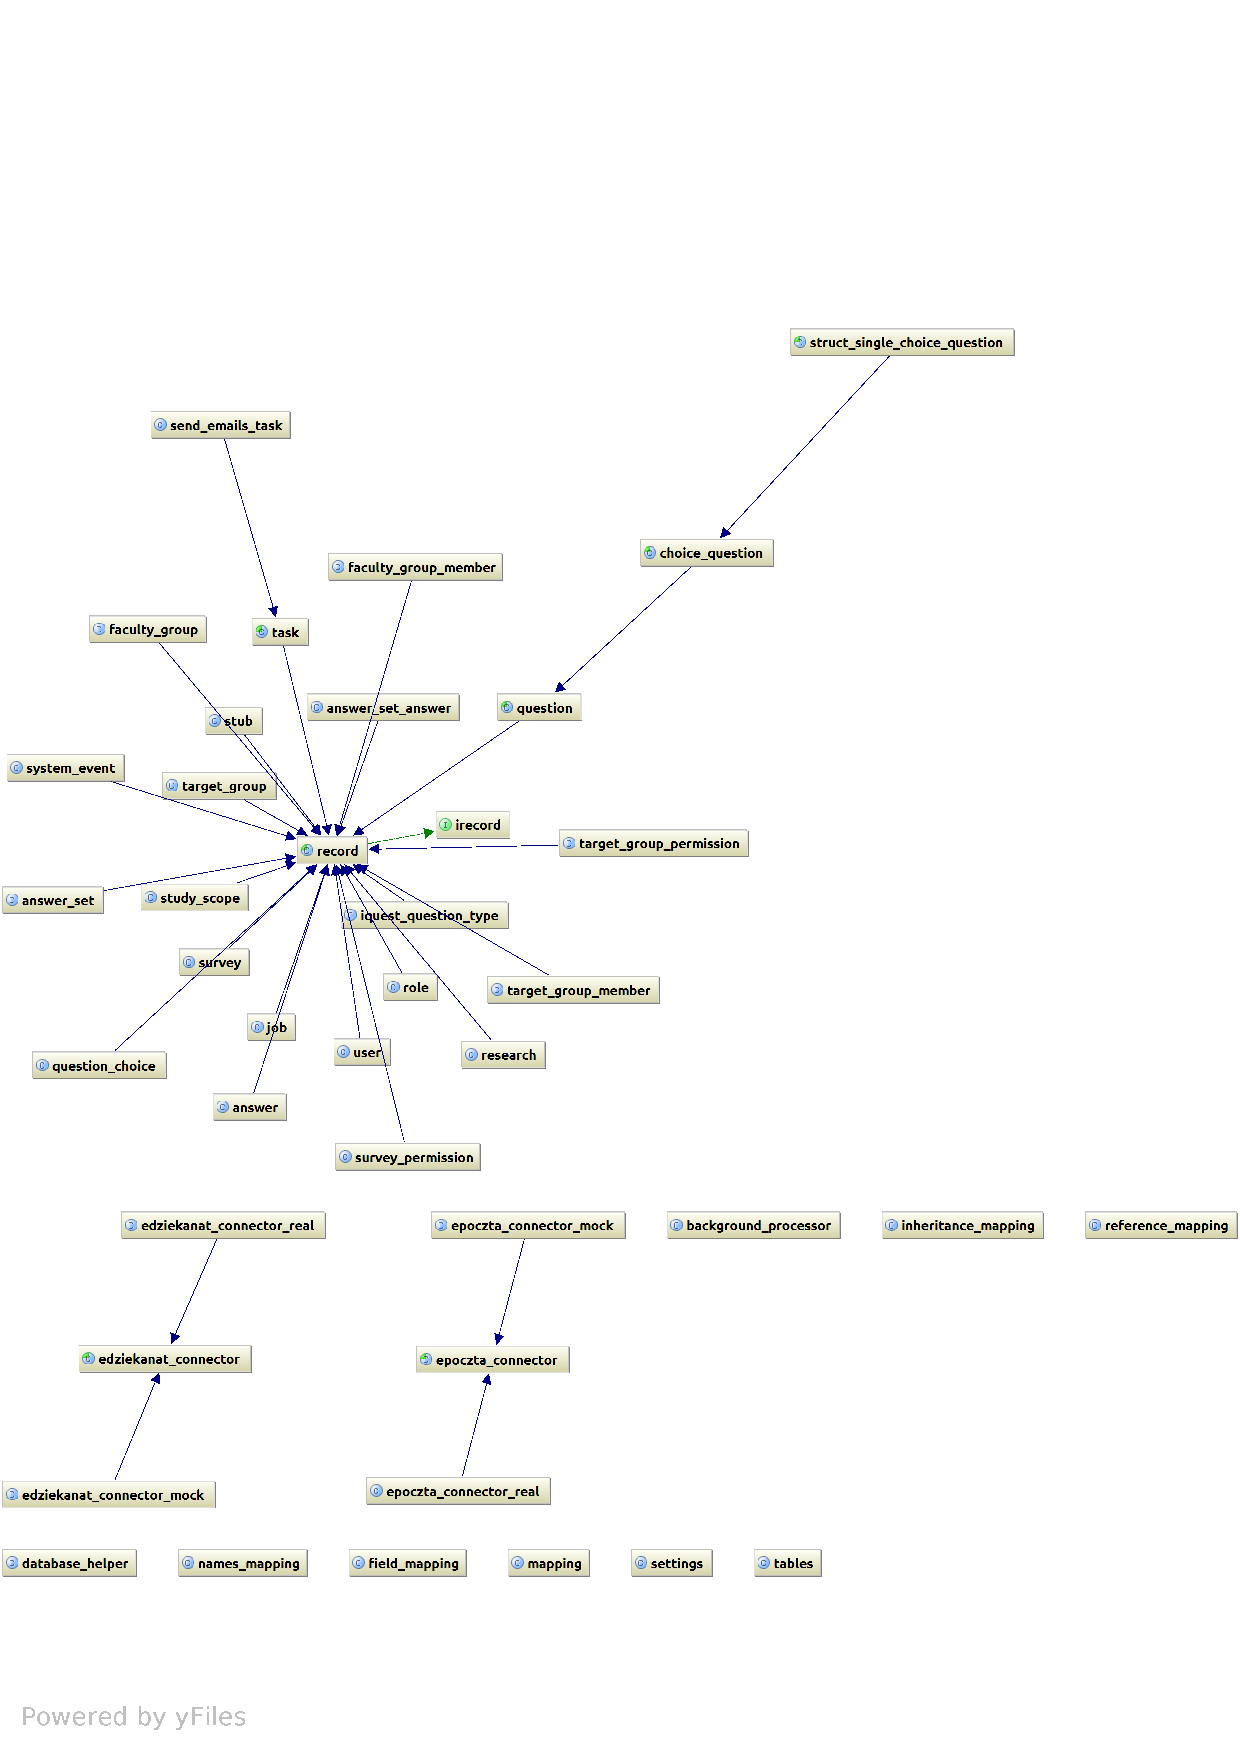
\includegraphics[width=0.9\textwidth]{figures/lw/backend.pdf} 
\end{center}
\caption{Struktura back-end'u}
\label{fig:back-end}
\end{figure}

\subsection{Raporty}
Raporty wykonano korzystając z platformy JasperReports, wykorzystując następujące produkty firmy \emph{Jaspersoft}:

\begin{itemize}
\item \emph{JasperReports Server} (wersja 5.0) -- serwer usług raportowania, na którym przechowywane są przygotowane przez zespół artefakty, w celu umożliwienia generacji raportu osobom dysponującym odpowiednimi uprawnieniami. Wykorzystano następujące funkcjonalności: definiowania źródła danych, raportu, ładowania plików z projektem raportu, zasobami oraz z generacji raportu.
\item \emph{Jaspersoft Studio} (wersja 1.3.2) -- bazowane na Eclipse narzędzie do projektowania raportów. Posłużyło zespołowi do przygotowania projektów raportów w formacie \emph{JRXML}.
\end{itemize}

Kody źródłowe pakietu \emph{JasperReports} są pisane w języku Java. Źródłem danych dla raportu, jest przygotowana przez zespół implementacja interfejsu \emph{ReportDataSourceService} z \emph{API JasperServer}. Źródło danych łączy się z udostępnianymi przez wskazaną instancję systemu \emph{iQuest} usługami zdalnymi, z których otrzymuje informacje o przeprowadzanych badaniach poprzez protokół SOAP. Struktura raportu zależy od typu pytania (otwarte/zamknięte). W przypadku pytań otwartych prezentowana jest lista odpowiedzi. Dla pytań zamkniętych na podstawie pobranych danych generowane są statystyki, które przekazywane są do podraportu w postaci obiektu klasy \emph{JRBeanCollectionDataSource}. W generacji statystyk z danych badań wykorzystano bibliotekę \emph{JoSQL}. Definicja projektu raportu składa się z czterech plików, odpowiadających trzem kolejnych poziomom:
\begin{enumerate}
\item \emph{researches.jrxml} -- raport główny dla badań,
\item \emph{questions.jrxml} -- podraport pytań,
\item \emph{answers\_closed.jrxml} oraz \emph{answers\_open.jrxml} -- podraporty odpowiedzi. zamkniętych i otwartych.
\end{enumerate}
Do generacji namiastek obiektów zdalnych (ang. \definicja{stub}) wykorzystano Apache Axis. Wygenerowane klasy dostosowano tak, by akceptowały obiekty z zadanej instancji \emph{iQuest} oraz dla zmiennej przestrzeni nazw (ang. \emph{namespace}).\\

W trakcie generacji \emph{stub'ów} okazało się, iż definicja usług dla protokołu \emph{SOAP} w języku \emph{WSDL} (\emph{Web Service Description Language}) generowana przez \emph{Moodle} jest niepoprawna. Skorzystano zatem z poprawionej wersji z zewnętrznego źródła (\url{https://github.com/ghigio/moodle-webservice_soapfda}).\\

Dostęp do usług zdalnych definiowanych w \emph{Moodle} zabezpieczono korzystając z mechanizmu generacji tokenu dla wybranego użytkownika. Użytkownik, który z poziomu serwera \emph{Jasper Server} zamierza wygenerować raport, musi znać adres naszego systemu oraz posiadać token dostępu do usługi.

\subsection{Moduły uwierzytelniania}
Korzystając z mechanizmów rozszerzeń \emph{Moodle} zaimplementowano dwa moduły uwierzytelniania, tj.:
\begin{itemize}
\item \emph{eKontoAuthenticationPlugin} -- integruje logowanie przez \emph{eKonto} z naszym systemem,
\item \emph{emailgraduate} -- pozwala absolwentom uczelni na rejestrację z użyciem adresu e-mail.
\end{itemize}

W celu spełnienia wymagań Działu Rozwoju Oprogramowania Politechniki Poznańskiej odnośnie wygaszania sesji użytkownika \emph{eKonto} po zadanym czasie (e.g. 15 min.) zmodyfikowano pliki źródłowe \emph{Moodle}, gdyż dla kodu odnoszącego się do sesji użytkownika \emph{Moodle} nie została przewidziana możliwość rejestracji rozszerzeń. Relacja \emph{user} została rozszerzona o opcjonalne pola związane z \emph{eKonto}, jako że kod odpowiedzialny za manipulację schematem bazy danych nie jest wykonywany podczas instalacji modułu uwierzytelniania, umieszczono go w osobnym module (\emph{ekontodb}). \emph{eKontoAuthenticationPlugin} może być instalowany bez konieczności instalacji \emph{iSurvey}. Podczas jego implementacji korzystaliśmy z dokumentu \emph{Centralne uwierzytelnianie i wymiana danych. Wersja 1.2 (2010.07.06)}.\\

Podczas rejestracji z użyciem naszych modułów użytkownik jest przydzielany do grupy docelowej ,,Absolwenci'', nadawana jest mu też rola respondenta w kontekście \emph{kursu iQuest}. Utworzenie modułu wiąże się z przygotowaniem klasy dziedziczącej z \emph{auth\_plugin\_base}, formularza ustawień, pliku lokalizacji oraz wersji.

\subsection{Moduły dla serwisów zewnętrznych}
\begin{itemize}
\item \emph{ePocztaConnector} -- służy do wysyłania e-maili z serwera Politechniki Poznańskiej,
\item \emph{eDziekanatConnector} -- pobiera i aktualizuje lokalne informacje o grupach dziekańskich, zakresach tematycznych tychże grup oraz ich studentach.
\end{itemize}

\emph{Dział Rozwoju Oprogramowania} udostępnia klienty \emph{eUsług} dla różnych języków, w tym dla \emph{PHP}. Komunikacja z usługami zdalnymi uczelni odbywa się poprzez protokół SOAP. Wyżej wymienione moduły zaimplementowano z wykorzystaniem fabryki obiektów, która w zależności od trybu (testowy/produkcyjny) zwraca obiekt odpowiedniej klasy. Zadania związane z oba modułami są zlecane procesorowi zadań w tle.

%to poleci gdzieś indziej.
%\begin{landscape}

%\begin{figure}[!th]
%\centering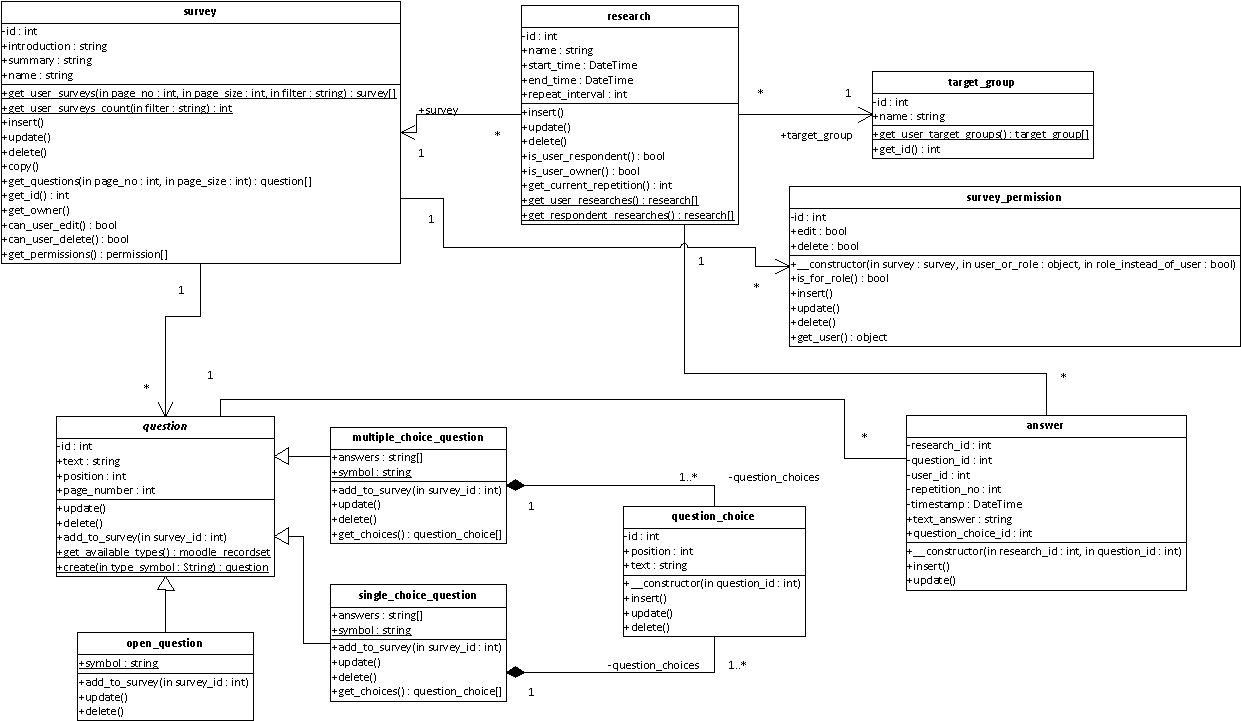
\includegraphics[width=1.25\textheight]{figures/Survey_Creator_Survey_Runner.png}
%\caption{Backend -- moduły Survey Creator i Survey Runner}\label{rys:iquest-backend}
%\end{figure}

%\begin{figure}[!th]
%\centering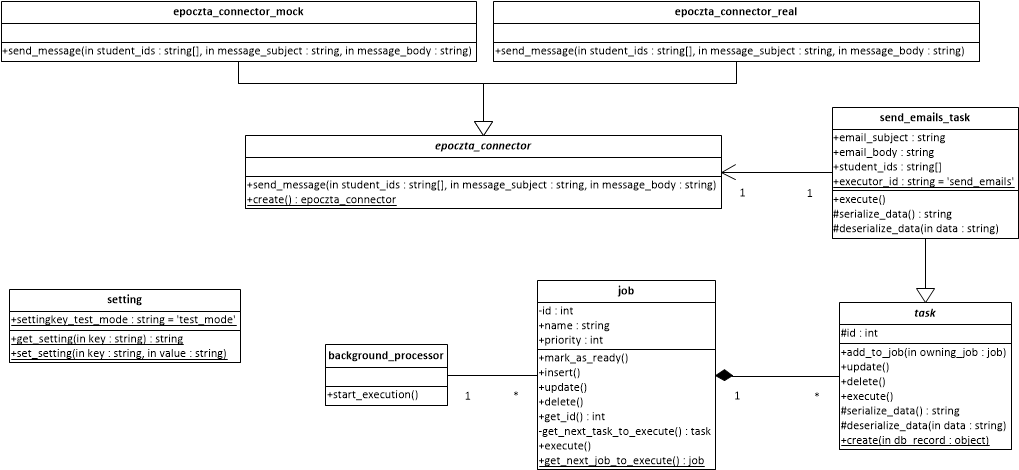
\includegraphics[width=1.25\textheight]{figures/ePoczta_Connector_Background_Task_Scheduler_and_Executor.png}
%\caption{Backend -- moduły ePoczta Connector i Background Task Scheduler and Executor}\label{rys:iquest-backend2}
%\end{figure}

%\end{landscape}

\section{Powiązanie back-endu z interfejsem}
\label{Chapter67}

%brak treści?

{\color{red}Koniec fragmentu niezredagowanego}